\chapter{Development of methods for tracking neurons and behavior over days}

\section{Introduction}
Significant technical limitations have prevented direct measurements of single cell activity-behavior relationships over long timescales, during stable behavior and during learning. To study how single cell response properties are modified or maintained over days and weeks, it is necessary to 1) measure the activity of the same neurons over time, 2) to do this in a behaviorally-relevant context, that is during a behavioral task. Recent technical advances in optical recording methods and head-fixed behavioral task design have satisfied these experimental demands.

\bigskip

Optical recording methods are additionally advantageous compared to electrical recording methods as they are more comprehensive and less invasive. Our brain region of interest, cortex, is located on the surface of the brain, thus optical access can be achieved in the intact brain. Compared to single or multiunit electrodes, this method is far less invasive, which will be important for long term recordings where tissue damage may cause changes in neuronal response properties. Optical recording methods are more comprehensive as a larger area of neurons may be recorded simultaneously. Additionally the experimenter can identify the fraction of active neurons using optical methods, whereas in electrical recordings silent neurons are missed. Although we didn't take advantage of cell type information in these studies, additional information using genetic markers can be incorporated into future work through the use of additional fluorescent markers.

\subsection{Two photon microscopy}
The development of multi-photon fluorescence microscopy has allowed for high resolution, high sensitivity measurement of fluorescent probes in light scattering tissue, up to 1 mm deep (1990 Denk et al)(Beaurepaire et al., 2001 ;  Theer et al., 2003). This system works through the combination of two low energy photons exciting one fluorescent molecule simultaneously, resulting in a transition to a higher energy state and a higher energy emission than would be possible from a single photon. This type of absorption scales with the second power of the light intensity, which drops off quadratically above and below the focal plane. As a result this is a nonlinear process, providing high resolution excitation within $ \approx $ 0.1 $ \mu m^3 $ (zipfel 2003). The use of low energy excitation light lessens the extent of photodamage in the tissue and allows for deeper penetration of excitation light due to reduced levels of scattering. Light is scattered in the tissue throughout both the excitation path and the emission path (half of photons are scattered every 50-200 $\mu$ m  (Oheim et al., 2001; Yaroslavsky et al., 2002 ;  Kleinfeld et al., 1998). Light scattered on the excitation path reduces light intensity in the focal region, but doesn't result in off-target excitation due to the low probability of two scattered photons simultaneously hitting the same fluorescent probe. Therefore, the source of all collected emission photons is the focal excitation volume and can be incorporated into the signal. This combination of high resolution excitation and blanket emission signal contribution allows high resolution and high sensitivity measurement of fluorescent probes in light scattering tissue.

\subsection{Fluorescent indicators}
More recent developments in fluorescent probes for neuronal activity have dramatically improved the signal strength and temporal resolution of optical recording methods. The local concentration of calcium ions rises between 10 and 100 fold in the soma during an action potential due to the opening of voltage gated calcium channels, making calcium ion concentration a good measure of activity(Berridge 2000). Structure guided optimization of the calcium sensor GCaMP, the circularly permuted green fluorescent protein linked to the calcium binding protein calmodulin, has rendered this complex the most widely used calcium sensor. The latest version of GCaMP was identified through a large scale genetic screen in neurons with the aim of improving sensitivity. GCaMP6 includes three variants, differing in their sensitivity and kinetics. All of these variants, (fast, medium and slow describe the off-rate of calcium binding) are reported to identify single spikes in vivo with signal strength inversely proportional to their off-rate. We chose to use GCaMP6m (medium) as the signal strength is nearly as high as GCaMPs (slow), with a faster off rate.  Various versions of GCaMP have already been used to detect neural activity in large neuronal populations in the PPC 8, motor cortex 66, barrel cortex 68, and hippocampus 7 of behaving mice. Long-term imaging of GCaMP has revealed learning-related circuit changes in vivo 65. Despite these advances, there are still limitations of these recording tools. Calcium indicators lack information about the relative event rate across neurons and blur the response timing of neurons. Calcium indicators also bias sampled activity to higher firing rates because small spike numbers can be missed (Druckmann Svoboda).

\bigskip

There are two options for the induction calcium indicator expression in vivo: virus-based lentiviral vector system and transgenic mouse lines. Long term viral expression provides superior signal to noise than current transgenic lines, although expression is variable across cells and is unstable over time, eventually leading to nuclear expression of the indicator and cell death. Transgenic lines do not have similar cell health problems and require a less invasive surgical procedure without the need for injections. However, expression levels in transgenic mice are low, resulting in poor signal to noise. Additionally one leading GCaMP6 transgenic line is reported to cause seizures in mice. Consequently, viral expression of calcium indicators is still the most widely implemented method for the induction of calcium expression. While the majority of cells display no aberrant response properties over the course of 1-2 months, careful measures must be taken to exclude unhealthy cells, which are conveniently labeled by nuclear expression of the indicator. This feature of virally expressed calcium indicators remains a source of concern and should be considered in the interpretation of our results.

\bigskip

An additional fluorescent protein that provides a stable image, independent from calcium responses, is useful for image registration across a single session and for field of view alignment across days. We additionally express the red fluorescent protein tdTomato in conjunction with the calcium indicator GCaMP6m.

\subsection{Developments in image processing}
Rapid advances in these technologies require matched developments in processing methods. There are three standard steps of image processing, 1) image registration across frames, 2) segmentation of fluorescent sources and 3) deconvolution to recover spiking information. Pipelines for these steps are often designed ad hoc and are specific to the indicator and acquisition methods of individual experimenters. Image processing techniques for these data are still in infant stages, although there has been a large amount of progress in the past decade. 

\bigskip

Two-photon excitation microscopes acquire single pixel intensities sequentially by scanning focused laser pulses across the imaging plane. Small displacements in the target tissue due to brain motion result in nonuniform distortions of the image. These distortions can often be reduced post hoc through image registration methods. Optimal registration methods incorporate statistics of acquisition methods into the design of the registration algorithm. For example, line scans result in a smaller temporal difference between horizontally adjacent pixels than vertically adjacent pixels. The Lucas Kanade method capitalizes on this piece of information to correct for distortion within a frame. Segmentation and deconvolution methods are also developing quickly. Coordinated competitions for data processing methods with ground truth data, such as codeneuro, will be crucial for the widespread acceptance and application of verified methods.

\subsection{Surgical methods for optical access to brain tissue}
These optical tools allow unprecedented access to the most superficial brain regions, specifically cerebral cortex, literally 'brain bark'. Utilization of these tools requires the partial removal of the overlying bone. This is achieved either through thinning the bone or by permanently replacing bone with glass. Both the thinned skull and the cranial window prep can lead to inflammation and microglia activation. Careful surgical technique is required to minimize the disruption of tissue (Dorand 21014, Xu et al). The cranial window surgery requires drilling down to very thin layers of bone without heating up or piercing brain tissue. The thinned skull prep is similarly difficult, where the appropriate bone thickness is 20 - 25 $\mu$ m directly above the target imaging region. Chronic recordings the through thinned skull are made difficult by skull irregularities, regrowth and repeated skin closure and resections. Approximately five days post-operation, bone regrowth occludes  brain tissue and the skull must be repeatedly thinned up to five times total (Yang G 2009). As a result cranial glass windows are the most widely accepted method for tracking the activity of neurons over days (Goldey 2014).

\subsection{The mouse as a model organism}
The combined advances in molecular and genetic tools and quantitative mouse behavior make mice the ideal model organism for studying neuronal population activity in relation to behavior. Careful quantitative behavior in mice is now on par with those in primates in terms of stimulus and behavioral control. A standard method in monkeys has been to head-fix and restrain the body of the animal. These methods allow careful measurement of unrestricted behavioral readouts, such as eye and arm position. New behavioral methods in rodents attempt to emulate these precision practices. A wide range of head fixed behaviors in mice have been developed over the past two decades. Mice have demonstrated perceptual capabilities for simple discrimination and decision making behaviors that have become increasingly complex. As in primate studies, mice are capable of performing hundreds of trials with performance approaching near perfect levels. Experiments in primates have laid the groundwork for quantitative analysis of neuronal activity in relation to behavior, however the the development of quantitative and conceptually rich mouse behavior in conjunction with rapid advancements of mouse specific molecular tools have rendered mice the ideal organism for future work in this area(O'Connor et al., 2009)(andermann 2010).

\subsection{A virtual reality system for mouse behavior}
The head fixed behavioral setup not only allows more precise stimulus control and precision measurements of motor outputs, but additionally allows implementation of advanced optical recording techniques. We use a head fixed behavior setup for the animal as in previous in vivo imaging studies 7,65. We use a navigational task as navigation is a natural decision making behavior for rodents. Our task employs a previously described virtual reality system 6. The mouse's running on a spherical treadmill controls translation and rotation a virtual environment. The virtual environment is projected onto a screen in a closed loop with the movements of the mouse. Mice are able to interact with the virtual environment, rapidly increasing their reward rate often within a single imaging session.

\subsection{Posterior parietal cortex}\label{methods:ppc}
An ideal brain area to study learned associations is the posterior parietal cortex because the PPC links sensory representations to a behavioral response. This sensorimotor association area is likely flexible during learning of new associations between sensory inputs and a motor response. PPC receives input from primary and secondary sensory areas and has extensive reciprocal connections with prefrontal association areas, frontal regions, limbic structures, as well as superior colliculus and basal ganglia53. PPC has been traditionally linked with spatial attention and movement planning 51,52. Involvement in cognitive functions such as working memory and task learning has become increasingly evident26. Lesions in PPC induce spatial attention and working memory deficits in humans. Typically after a lesion in the right hemisphere, patients will experience inability to detect objects in the contralateral visual hemisphere or to perceive the left side of objects, regardless of where they appear within the visual field. Balint?s syndrome is common in PPC lesion studies where patients are unable to perceive more than one visual stimulus at a time, to direct visual attention outside the fovea, to scan visual space, or to coordinate hand movements to visual targets54. Another role of the PPC is its function in receiving and integrating polymodal sensory information, and transforming it into goal-directed motor movements55?57. PPC is recognized for its role in motor learning and retrieval of learned complex motor skills 58?61. The precise role of PPC in the decision making circuit is somewhat controversial. Initial reports of working memory activity in the posterior parietal cortex described spiking in monkey area LIP that followed the offset of a visual stimulus, which was to be a target for a planned eye movement25. Later studies demonstrated that posterior parietal neurons represent the remembered locations of visual stimuli, independent of a planned motor response5,62,63. More recent work in rodent PPC have demonstrated a role for this association area during the cue period of visual decision making tasks, suggesting rodent PPC is involved in some form of visual processing or potentially the transformation of stimulus information into an action plan. PPC activity is working memory task modulated, linking sensory information and the behavioral response, making it an ideal focus for the study of learned cue-response relationships. This association area will serve as an example for learning and cortical processing in other association areas.

\bigskip

Functionally defined boundaries for higher order visual areas is an active area of investigation (recent neuron papers). The Allen Institute Mouse Brain Atlas provides a widely accepted map of cortical areas defined by connectivity. This map has been in flux over recent years, with subtle changes in cortical area boundaries in each new addition. We define our PPC coordinates 2 mm posterior and 1.7 mm lateral of bregma. We performed retinotopic mapping experiments to identify our stereotaxically defined PPC relative to functionally defined visual areas. These coordinates corresponded to a location anterior to cortical regions identified using retinotopic mapping. Here we note that recent work from the Allen Brain Institute calls this region VisA and that this region is medial to what previous work has called secondary visual area A.

\begin{figure}
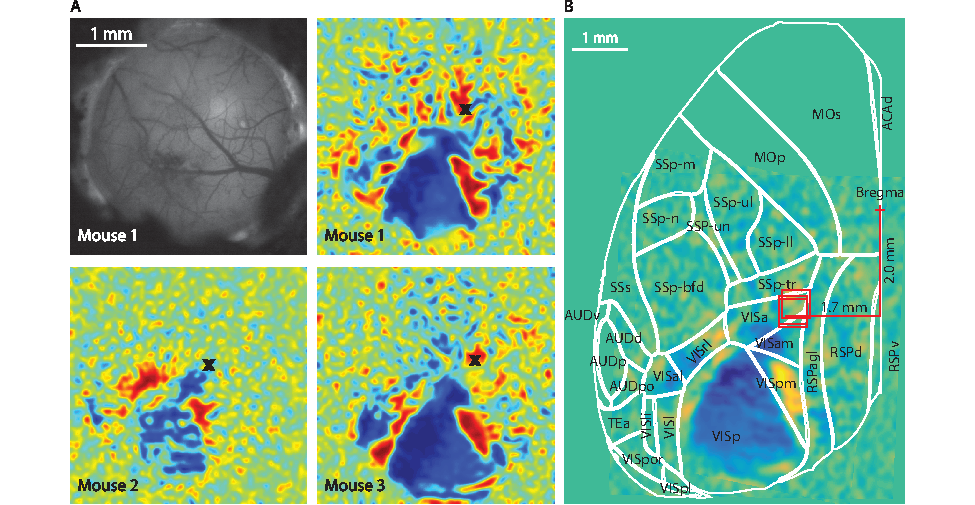
\includegraphics[width=\textwidth]{figures/widefield.pdf}
\caption[PPC relative to retinotopic maps]{\textbf{PPC relative to retinotopic maps. a,} Upper left: Blood vessel image through cranial window. Upper right and bottom panels : Field sign maps
%
\textbf{b,} Combined field sign maps overlayed with a dorsal map of cortical areas defined by the Allen Mouse Common Coordinate Framework.
\label{fig:widefield}}
\end{figure}

\section{Detailed methods for chronic recordings}

\subsection{Mice}
All experimental procedures were approved by the Harvard Medical School Institutional Animal Care and Use Committee and were performed in compliance with the Guide for the Care and Use of Laboratory Animals. Three male C57BL/6J-Tg(Thy1-GCaMP6s)GP4.12Dkim/J mice were used for widefield retinotopic mapping experiments, All other data were obtained from five male C57BL/6J mice (Jackson Labs), which were 8-10 weeks old at the start of behavioral training, and 14-32 weeks old during imaging. A surgery was performed on each mouse before training to affix a titanium headplate to the skull using dental cement (Metabond, Parkell). At least one day after headplate implantation, mice began a water schedule, in which they received 800 l of water/day. Mouse health was monitored daily. Mice were given additional water if their weight fell below 80 $\%$ of their pre-schedule weight (mean ± sem 23.2 ± 0.5 g). Mice were housed in pairs of littermates.

\subsection{Virtual environment design}
Virtual reality environments were constructed and operated using MATLAB-based ViRMEn software (Virtual Reality Mouse Engine) (Aronov and Tank, 2014; Harvey et al., 2009). A PicoP microprojector (MicroVision Inc.) projected the virtual environment onto the back side of a 24 inch diameter half cylindrical screen. The virtual environment was updated in response to the mouse's manipulations of an open cell Styrofoam spherical treadmill (8 inch diameter, ~135 g). An optical sensor positioned beneath the spherical treadmill measured movements in pitch and roll of the ball (relative to the mouse's body axis). These signals controlled forward/backward and rotational movement in VR, respectively. We recorded the mouse's position in the virtual environment (x/y position), the rotational speed of the spherical treadmill (about the pitch and roll axes), and the mouse's view angle in the environment. 

\subsection{Fixed association decision task}
We trained mice to perform a two-alternative forced-choice task based on navigation through a T-maze in visual virtual reality (Harvey et al., 2012). At the beginning of the T-stem, mice saw one of two possible visual cues (white walls or black walls). Mice then ran through a short delay period portion of the T-stem in which the walls were identical between trial types. Upon reaching the T-intersection, mice had to report a choice about the cue identity by making a left or right turn to receive a reward. Mice learned this task over 4-6 weeks of training and reached expert behavioral performance that was mostly stable over weeks.

\subsection{Training procedure} 
Mice were on the water schedule for at least five days before behavioral training began. Training sessions were performed daily and lasted 45-60 minutes at roughly the same time of day each day. Rewards (4 L of 10$\%$ sweetened condensed milk in water) were delivered through a lick spout. Mice were trained to perform the T-maze task using a program of five mazes. 

\bigskip

\subsubsection{2 cue task training}
Maze 1 was a linear track in which the mouse had to run forward to get a reward.  After each trial the maze was either lengthened or shortened to maintain an approximate reward rate of 4 rewards/minute. When the mouse completed a trial in less than 15 seconds, the central corridor would grow by 10 centimeters on the next trial or shrink by the same amount if the trial was completed in greater than 15 seconds. The minimum length of the maze was 37.5 cm and the maximum was 3 m (measured as running distance on the treadmill). 

\bigskip

In maze 2 the mice had to turn toward a tower above the left or right T-arm in the virtual world. This maze trained the mice to follow a visual cue for reward and improved running skill on the treadmill. Again, after each trial the maze was either lengthened or shortened to maintain an approximate reward rate of 4 rewards/minute with a minimum length of 70 cm and a maximum length of 3.5 m. 

\bigskip

In maze 3, mice began to associate colored walls with the cued turn direction. When the tower was on the right, the walls were black. When the tower was on the left, the walls were white. On alternating trials we added a second tower so that there was one on each side, and the mouse had to use the wall color to plan the turn direction. Maze 3 was 4 m in length. 

\bigskip

The delay period was gradually incorporated into maze 4, such that the cue offset (delay onset) shifted earlier in the trial. The criteria for advancement to the next maze in the sequence, on mazes 3 and 4, were a trial rate of > 4 trials/minute and > 80$\%$ correct for 2-3 consecutive days. 

\bigskip

In maze 5, the lengths were fixed with the total length of 4.5 m and a delay period of 2.25 m. The colored walls were either black with white dots or white with black dots followed by a gray striped segment throughout the delay period that was identical across trial types. The entire training program was completed in 4-8 weeks.

\bigskip

\subsubsection{3 and 4 cue task training}
Training for novel trial type associations was performed during imaging. Mazes were identical to maze 5. On each day, mice were presented with novel trial types after 40 trials of the original trial types (black cue-right turn and white cue-left turn). After novel trial types were introduced, familiar trial types and novel trial types were interleaved such that there were equal fractions of left and right turn trials. Mice were first presented with a 3rd cue (crosshatch) and after mice performed all three trial types at above 80$\%$ for three consecutive days, we introduced a 4th cue (triangles). For mouse 1, the 3rd cue instructed left turns and the 4th cue instructed right turns. For mouse 3, the cue-turn relationship for novel trial types was reversed. White and black cues maintained consistent cue-turn relationships for both mice. Mice learned novel trial type cue-turn relationships by trial and error while maintaining previously learned relationships for black and white cues. 

\bigskip

\subsubsection{Bias Correction}
Some mice developed biases during training such that left or right turns were favored. During training, we implemented a bias correction. On each trial, the probability that a mouse would be presented with a left turn trial was the fraction of times the mouse turned right on the previous 20 trials. Once mice reached expert levels, biases were rare and bias correction was unnecessary. Bias correction was not used during imaging sessions.

\subsection{Surgical procedures}
After mice achieved performance greater than 80$\%$ correct on the task for five consecutive days, they received ad lib access to water for three days before the cranial window implant surgery. A circular craniotomy with a diameter of 3.1 mm was made over left PPC (stereotaxic coordinates: 2 mm posterior, 1.7 mm lateral of bregma). Three 10 nL injections of a virus mixture containing a 4:1 volumetric ratio of tdTomato (AAV2/1-CAG-tdTomato) to GCaMP6m (AAV2/1-synapsin-1-GCaMP6m) (University of Pennsylvania Vector Core Facility) were made near the center of the craniotomy at a depth of ~275 $\mu$ m below the dura. Injections were slow (5 min/injection) and continuous (custom air pressure injection system). The pipette (15 $\mu$ m tip diameter) was advanced using a micromanipulator (Sutter MP285) at a 30-degree angle relative to horizontal to minimize compression of the brain. A glass plug consisting of a single 5 mm diameter coverslip on top of two 3 mm diameter coverslips ($\#$ 1 thickness; CS-5R and CS-3R, Warner Instruments) were combined using UV-curable optically transparent adhesive (Norland Optics) and were affixed to the brain with minimal Kwik-Sil (World Precision Instruments) and affixed to the skull using Metabond on the perimeter of the 5mm coverslip lip. The metabond mixture contained 5$\%$ vol/vol India ink, to prevent light contamination from the VR display. A titanium ring was mounted on top of the headplate. This ring interfaced with the objective lens through a cylinder of black rubber, to prevent light contamination (Dombeck et al., 2010). Mice resumed training after at least one day of recovery. Imaging began at least three weeks post-injection and was continued for up to 8 weeks. On a given day, we imaged 100 - 300 neurons simultaneously during approximately 200 trials.

\subsection{Field sign maps}
To visualize Bregma guided PPC coordinates relative to the retinotopic map in visual areas of the mouse cortex, we performed widefield imaging in GCaMP6s transgenic mice (C57BL/6J-Tg(Thy1-GCaMP6s)GP4.12Dkim/J) during a stimulus protocol for retinotopic mapping.

\subsubsection{Widefield microscope design}
Retinotopic mapping was performed with a tandem-lens epifluorescence macroscope (Ratzlaff and Grinvald, 1991). Excitation light (455 nm LED, Thorlabs) as filtered (469 nm with 35 nm bandwidth, Thorlabs) and reflected onto the brain through an inverted camera lens (NIKKOR AI-S FX 50 mm f/1.2, Nikon). Emission light was collected by the same lens, emission-filtered (525 nm with 39 nm bandwidth, Thorlabs), and imaged by a second camera lens (SY85MAE-N 85 mm F1.4, Samyang) onto a CMOS camera (ace acA1920-155um, Basler). Images were collected at 60 Hz, synchronized to the visual stimulus presented on a gamma-corrected 27 inch IPS LCD monitor (MG279Q, Asus). 

\subsubsection{Visual stimulus design}
Stimulation was performed as described in (Marshel et al., 2011). The monitor was placed in front of the right eye at an angle of 30 degrees from the mouse’s midline. The stimulus was a black and white checkered moving bar on a gray background, corrected to have constant width (5 degrees) and speed (7 degrees per second) in spherical coordinates centered on the mouse’s eye as described in (Marshel et al., 2011). The stimulus was presented in blocks containing 6 repeats of each of four movement directions (up, down, forward, backward). 6 blocks were presented per session. 

\subsubsection{Retinotopy analysis design}
Retinotopy was determined by computing the temporal Fourier transform at each pixel and extracting the phase at the frequency of stimulus presentation, as described in (Kalatsky and Stryker, 2003). The phase images were averaged across all trials of the same orientation and smoothed using a Gaussian kernel with standard deviation 30 $\mu$ m to obtain horizontal and vertical retinotopic maps. The field sign map was then calculated as the sine between the gradient angles of the horizontal and vertical retinotopic maps (Garrett et al., 2014; Sereno et al., 1994). Field sign maps were aligned to Allen Institute field sign maps using control point registration and overlaid with a dorsal map of cortical areas defined by the Allen Mouse Common Coordinate Framework(Mouse and Coordinate, 2015)

\subsection{Two photon microscope design} 
Data were collected using a custom-built two-photon microscope. A resonant scanning mirror and galvanometric mirror separated by a scan lens-based relay telescope on the scan head allowed fast scanning. A Olympus 25x 1.05 NA objective lens was mounted on a piezo collar (Physik Instrumente) that allowed slower axial scanning. An aluminum box housed collection optics to block light interference from the VR display. Green and red emission light were separated by a dichroic mirror (580 nm long-pass, Semrock) and bandpass filters (525/50 and 641/75 nm, Semrock) and collected by GaAsP photomultiplier tubes (Hamamastu). A Ti:sapphire laser (Coherent) delivered excitation light at 920 nm with an average power of about 35-70 mW at the sample. The microscope was controlled by ScanImage (version 4; Vidrio Technologies) (Pologruto et al., 2003). The spherical treadmill was mounted on an XYZ translation stage (Dover Motion) to position the mouse under the objective.

\subsection{Image acquisition}
Four imaging planes were acquired by volumetric scanning at 5.3 Hz with a resolution of 512 x 512 pixels (500 $\mu$ m x 500 $\mu$ m) for each plane. Planes were separated by 25 $\mu$ m axially between 120 and 250 $\mu$ m below the dura. Imaging was continuous over behavioral sessions lasting 45 minutes to 1 hour. Bleaching of GCaMP6m was negligible over this time. Approximately every 20 minutes, slow drifts of the field of view were manually corrected using comparison to a reference image. The imaging frame clock and an iteration counter in ViRMEn were recorded to synchronize imaging and behavioral data.

\subsection{Processing of imaging data}
One field-of-view was acquired for each of the five mice over a period of 3 to 8 weeks. The same plane was identified on consecutive days using coarse alignment based on superficial blood vessels followed by careful alignment to reference images at various levels of magnification in the red channel (using tdTomato expression). AAV-mediated expression of GCaMP6m provides high signal-to-noise compared to other methods; however, viral expression is known to increase over months which can lead to compromised signal over time, which is correlated with nuclear localization of the indicator (Chen et al., 2013; Tian et al., 2009). For this reason, imaging was discontinued when fields-of-view contained several cells with GCaMP6 in the nucleus, and all cells with nuclear localization were excluded from analysis (Supplementary Figure S2I). These methods are in accordance with other long-term imaging studies (Huber et al., 2012). Event rates of all analyzed cells were stable across time along with other properties of the population activity (Figure 5). Moreover, our ability to model and predict neuronal activity using behavioral features remained consistent throughout the duration of this experiment. For these reasons we have no reason to believe cell health was an issue in this work. 

\subsection{Within-session processing}
We implemented custom-written MATLAB software for streamlined motion correction, definition of putative cell bodies, and extraction of fluorescence traces. Following motion correction based on the Lucas-Kanade method (Greenberg and Kerr, 2009), putative cell bodies were first identified by eye and then binary masks were calculated based on the correlation of fluorescence timeseries between pairs of pixels located within 60 $\mu$ m of one another in the neighborhood of the identified cell. A continuous-valued, eigenvector-based approximation of the normalized cuts objective (Shi and Malik, 2000) was applied to the pixel correlation matrix, followed by discrete segmentation using k-means clustering. A separate neuropil mask was identified to accompany each cell body, defined using the same normalized cuts and segmentation method. Neuropil contamination was removed from the cell fluorescence time series by subtracting the background time series scaled by a contamination factor. The contamination factor was calculated by regressing the cell fluorescence against the background time series (Supplementary Figure S2E). ROI selection and neuropil subtraction were manually verified and manipulated when necessary using an interface tool that allowed examination of anatomical information and fluorescence traces corresponding to each cluster. The event rate was estimated using a previously described autoregressive deconvolution algorithm (Vogelstein et al., 2010) to minimize the impact of indicator kinetics. This metric describes the relative firing rate of each neuron over time but cannot be used to confidentially identify single spikes. We therefore refer to deconvolved traces as an estimated event rate.

 \subsection{Across-session processing}\label{methods:across days}
Binary masks for all fluorescence sources were identified on each day separately and then aligned across days using a semi-automated custom tool. The algorithm ranked cells across imaging days with their most likely matches based on proximity after alignment and anatomical image correlation (a 60 $\mu$ m box around the centroid of the cell). Matches were then verified by eye. This method has advantages over other commonly used approaches. Other approaches often use a single map of ROI masks for all days, such that this map is transformed on each day to best fit that day's imaging alignment. Slight deviations in the axial plane of the image or other sources of in-plane distortion could lead to slight offsets in masks from day-to-day relative to the ideal mask. Such slight offsets could result in contamination from activity in other cells, dendrites, and axons. Our approach identifies signal sources on each day and thus avoids any potential contamination from other signal sources. We then align the signal sources identified on each day to those from other days. The only error that could result is in incorrectly calling two signal sources as the same across days. However, to prevent such errors we visually compared the anatomical images to make sure the signal sources appeared to correspond to the same cell. If a cell could not be confidently identified on a given day, the data were excluded on that day. As a result, our approach resulted in an incomplete map of all cells across all days. We note that cells had to have some activity (calcium transients) in order to be identified on a given day. This activity requirement for the identification of each cell could potentially result in an underestimation in the extent to which cells gain and lose task related activity. Cells were more likely to have a defined mask on days that were nearby in time due to variable activity and viral expression of the indicator GCaMP6m (Figure \ref{fig:cell_selection} j). 

\begin{FPfigure}
\includegraphics[width=\textwidth,center]{figures/cell_selection.pdf}
\caption[Cell identification protocol across days and number of samples for various day comparisons.]
{\textbf{Cell identification protocol across days and number of samples for various day comparisons. a,} Fluorescence image of a 60 μm neighborhood of cells.
%
\textbf{b,} Correlation matrix between the time series of pixel values within the 60 $\mu$ m neighborhood.
%
\textbf{c,} Segmentation of pixels within 60 $\mu$ m neighborhood.
%
\textbf{d,} Mean fluorescence time series of pixels within each segment.
%
\textbf{e,} ROI fluorescence is regressed against background fluorescence. A neuropil contamination factor is the slope of the best fit line using bottom 8th percentile of ROI fluorescence (red).
%
\textbf{f,} Top: ROI fluorescence, bottom 8th percentile labelled in red. Middle: Neuropil fluorescence. Bottom: ROI fluorescence with (contamination factor * background) subtracted.
%
\textbf{g,} ROI maps found using protocol in panels \textbf{a-f} from two example imaging days.
%
\textbf{h,} Top: Overlay of average fluorescence signal from the example imaging days before and after registration based on intensity of tdTomato expression. Bottom: ROI outlines found using protocol in panels \textbf{a-f} before and after image registration using the transform from fluorescence image alignment.
%
\textbf{i,} Seven example cells across all imaging days with identified matches.
%
\textbf{j,} Left: Number of cells with good matches identified on each imaging day for each mouse. Middle: Cumulative distribution of number of imaging days with good matches for all cells in each mouse. Right: Probability that a cell was identified with a good match on two days separated by various intervals. 
%
\textbf{k,}Left: Number of mice with data on each imaging day. Middle: Number of mice with data on two days separated by various intervals. Right: Number of mice with data for each day comparison.
\label{fig:cell_selection}}
\end{FPfigure}
%\afterpage{\clearpage}
\clearpage

\bigskip